% -----------------------------------------------
% Template for SMC 2016
% adapted from the template for SMC 2012 and 2011, which were adapted from that of SMC 2010
% -----------------------------------------------

\documentclass{article}
\usepackage{smc2017}
\usepackage{times}
\usepackage{ifpdf}
\usepackage[english]{babel}
\usepackage{cite}

%%%%%%%%%%%%%%%%%%%%%%%% Some useful packages %%%%%%%%%%%%%%%%%%%%%%%%%%%%%%%
%%%%%%%%%%%%%%%%%%%%%%%% See related documentation %%%%%%%%%%%%%%%%%%%%%%%%%%
%\usepackage{amsmath} % popular packages from Am. Math. Soc. Please use the 
%\usepackage{amssymb} % related math environments (split, subequation, cases,
%\usepackage{amsfonts}% multline, etc.)
%\usepackage{bm}      % Bold Math package, defines the command \bf{}
%\usepackage{paralist}% extended list environments
%%subfig.sty is the modern replacement for subfigure.sty. However, subfig.sty 
%%requires and automatically loads caption.sty which overrides class handling 
%%of captions. To prevent this problem, preload caption.sty with caption=false 
%\usepackage[caption=false]{caption}
%\usepackage[font=footnotesize]{subfig}


%user defined variables
\def\papertitle{\textit{Live Orchestral Piano}, a system for real-time orchestral music generation}
\def\firstauthor{L\'eopold Crestel}
\def\secondauthor{Philippe Esling}
\def\thirdauthor{Third author}

% adds the automatic
% Saves a lot of ouptut space in PDF... after conversion with the distiller
% Delete if you cannot get PS fonts working on your system.

\usepackage[pdftex,
pdftitle={\papertitle},
pdfauthor={\firstauthor, \secondauthor, \thirdauthor},
bookmarksnumbered, % use section numbers with bookmarks
pdfstartview=XYZ % start with zoom=100% instead of full screen; 
                 % especially useful if working with a big screen :-)
]{hyperref}
%\pdfcompresslevel=9

\usepackage[pdftex]{graphicx}
% declare the path(s) where your graphic files are and their extensions so 
%you won't have to specify these with every instance of \includegraphics
\graphicspath{{../Figures/}}
\DeclareGraphicsExtensions{.pdf,.jpeg,.png}

\usepackage[figure,table]{hypcap}



% % % % % % % % % % %
% % % % % % % % % % %
% % % % % % % % % % %

\usepackage{amsmath,amssymb} % For including math equations, theorems, symbols, etc
\usepackage{bm}
\usepackage{graphicx} % Required for including images
\graphicspath{{../Figures/}} % Set the default folder for images
\usepackage{prettyref}
% Makecell 
\usepackage{makecell}
\renewcommand\theadalign{cb}
\renewcommand\theadfont{\bfseries}
\renewcommand\theadgape{\Gape[4pt]}
\renewcommand\cellgape{\Gape[4pt]}

% % % % % % % % % % %
% % % % % % % % % % %
% % % % % % % % % % %



%setup the hyperref package - make the links black without a surrounding frame
\hypersetup{
    colorlinks,%
    citecolor=black,%
    filecolor=black,%
    linkcolor=black,%
    urlcolor=black
}


% Title.
% ------
\title{\papertitle}

%Two addresses
%--------------
 \twoauthors
   {\firstauthor} {IRCAM \\ %
     {\tt \href{mailto:leopold.crestel@ircam.fr}{leopold.crestel@ircam.fr}}}
   {\secondauthor} {IRCAM \\ %
     {\tt \href{mailto:philippe.esling@ircam.fr}{philippe.esling@ircam.fr}}}


% ***************************************** the document starts here ***************
\begin{document}
%
\capstartfalse
\maketitle
\capstarttrue
%
\begin{abstract}
This paper introduces the first system for performing automatic \textit{orchestration} based on a real-time piano input. We believe that it is possible to learn the underlying regularities existing between piano scores and their orchestrations by notorious composers, in order to automatically perform this task on novel piano inputs. To that end, we investigate a class of statistical inference models based on the \textit{Restricted Boltzmann Machine} (\textit{RBM}). We introduce a specific evaluation framework for orchestral generation based on a prediction task in order to assess the quality of different models. To gain a better understanding of these quantitative results, we provide a qualitative analysis of the performances of the models, from which we try to extract the most crucial features of amongst the different architectures. As prediction and creation are two widely different endeavours, we discuss the potential biases in evaluating temporal generative models through prediction tasks and their impact on a creative system. Finally, we introduce an implementation of the proposed models called \textit{Live Orchestral Piano} (LOP), which allows to perform real-time projective orchestration of a MIDI keyboard input.
\end{abstract}
%


\section{Introduction}
% Orchestration classique
%% Musical orchestration : why is it so hard ?
% Orchestration
\textit{Orchestration} is the subtle art of writing musical pieces for the orchestra, by combining the properties of various instruments in order to achieve a particular sonic rendering \cite{koechli_orch,Rimsky-Korsakov:1873aa}. Because it extensively relies on spectral characteristics, orchestration is often referred to as the art of manipulating instrumental timbres \cite{mcadams2013timbre}. Timbre is defined as the property which allows listeners to distinguish two sounds produced at the same pitch and intensity.
% -> Timbre
Hence, the sonic palette offered by the pitch range and intensities of each instrument is augmented by the wide range of expressive timbres produced through the use of the different playing styles.
% Non linear spectral behaviours
Furthermore, it has been shown that some instrumental mixtures can not be characterized by a simple summation of their spectral components, but can lead to a unique \textit{emerging timbre}, with phenomenon such as orchestral blend \cite{tardieu2012perception}.
% -> Combinatoire
Given the number of different instruments in a symphonic orchestra, their respective range of expressiveness (timbre, pitch and intensity), and the phenomenon of emerging timbre, one can foresee the extensive combinatorial complexity embedded in the process of orchestral composition.

\textbf{Those difficulties have been a major obstacle towards the construction of a scientific basis for the study of orchestration. From a mathematical point of view, it seems that no set of descriptors can exhaustively fit with the perceptual complexity of timbre \cite{peeters2011timbre}. From a musical point of view, there is a lack of specific symbolic notation for timbre, and orchestration remains an empirical discipline taught through the observation of existing orchestration examples \cite{piston-orch}. //USELESS}

Among the different writing techniques for orchestral works, one of them consists in first writing an harmonic and rhythmic structure in the form of a piano score and then adding the timbre dimension by spreading the different voices over the various instruments \cite{piston-orch}. We refer to this operation of extending a piano draft to an orchestral score as \textit{projective orchestration} \cite{eslingthesis}.
The orchestral repertoire contains a large number of examples of projective orchestration (such as the piano reductions by Liszt of Beethoven symphonies or the \textit{pictures at an exhibition}, a piano piece by Moussorgsky orchestrated by Ravel among several notorious composers). By observing a case of projective orchestration (see \prettyref{fig:orch}), we can clearly see that this process involves more than the mere allocation of notes written on the piano score across the different instruments. It rather implies harmonic enhancements and timbre manipulations to underline the already existing harmonic and rhythmic structure \cite{mcadams2013timbre}. However, the visible correlations occurring at a local between a piano score and its orchestrations appear as a fertile framework for laying the foundations of a computational exploration of orchestration.

\begin{figure}
\centering
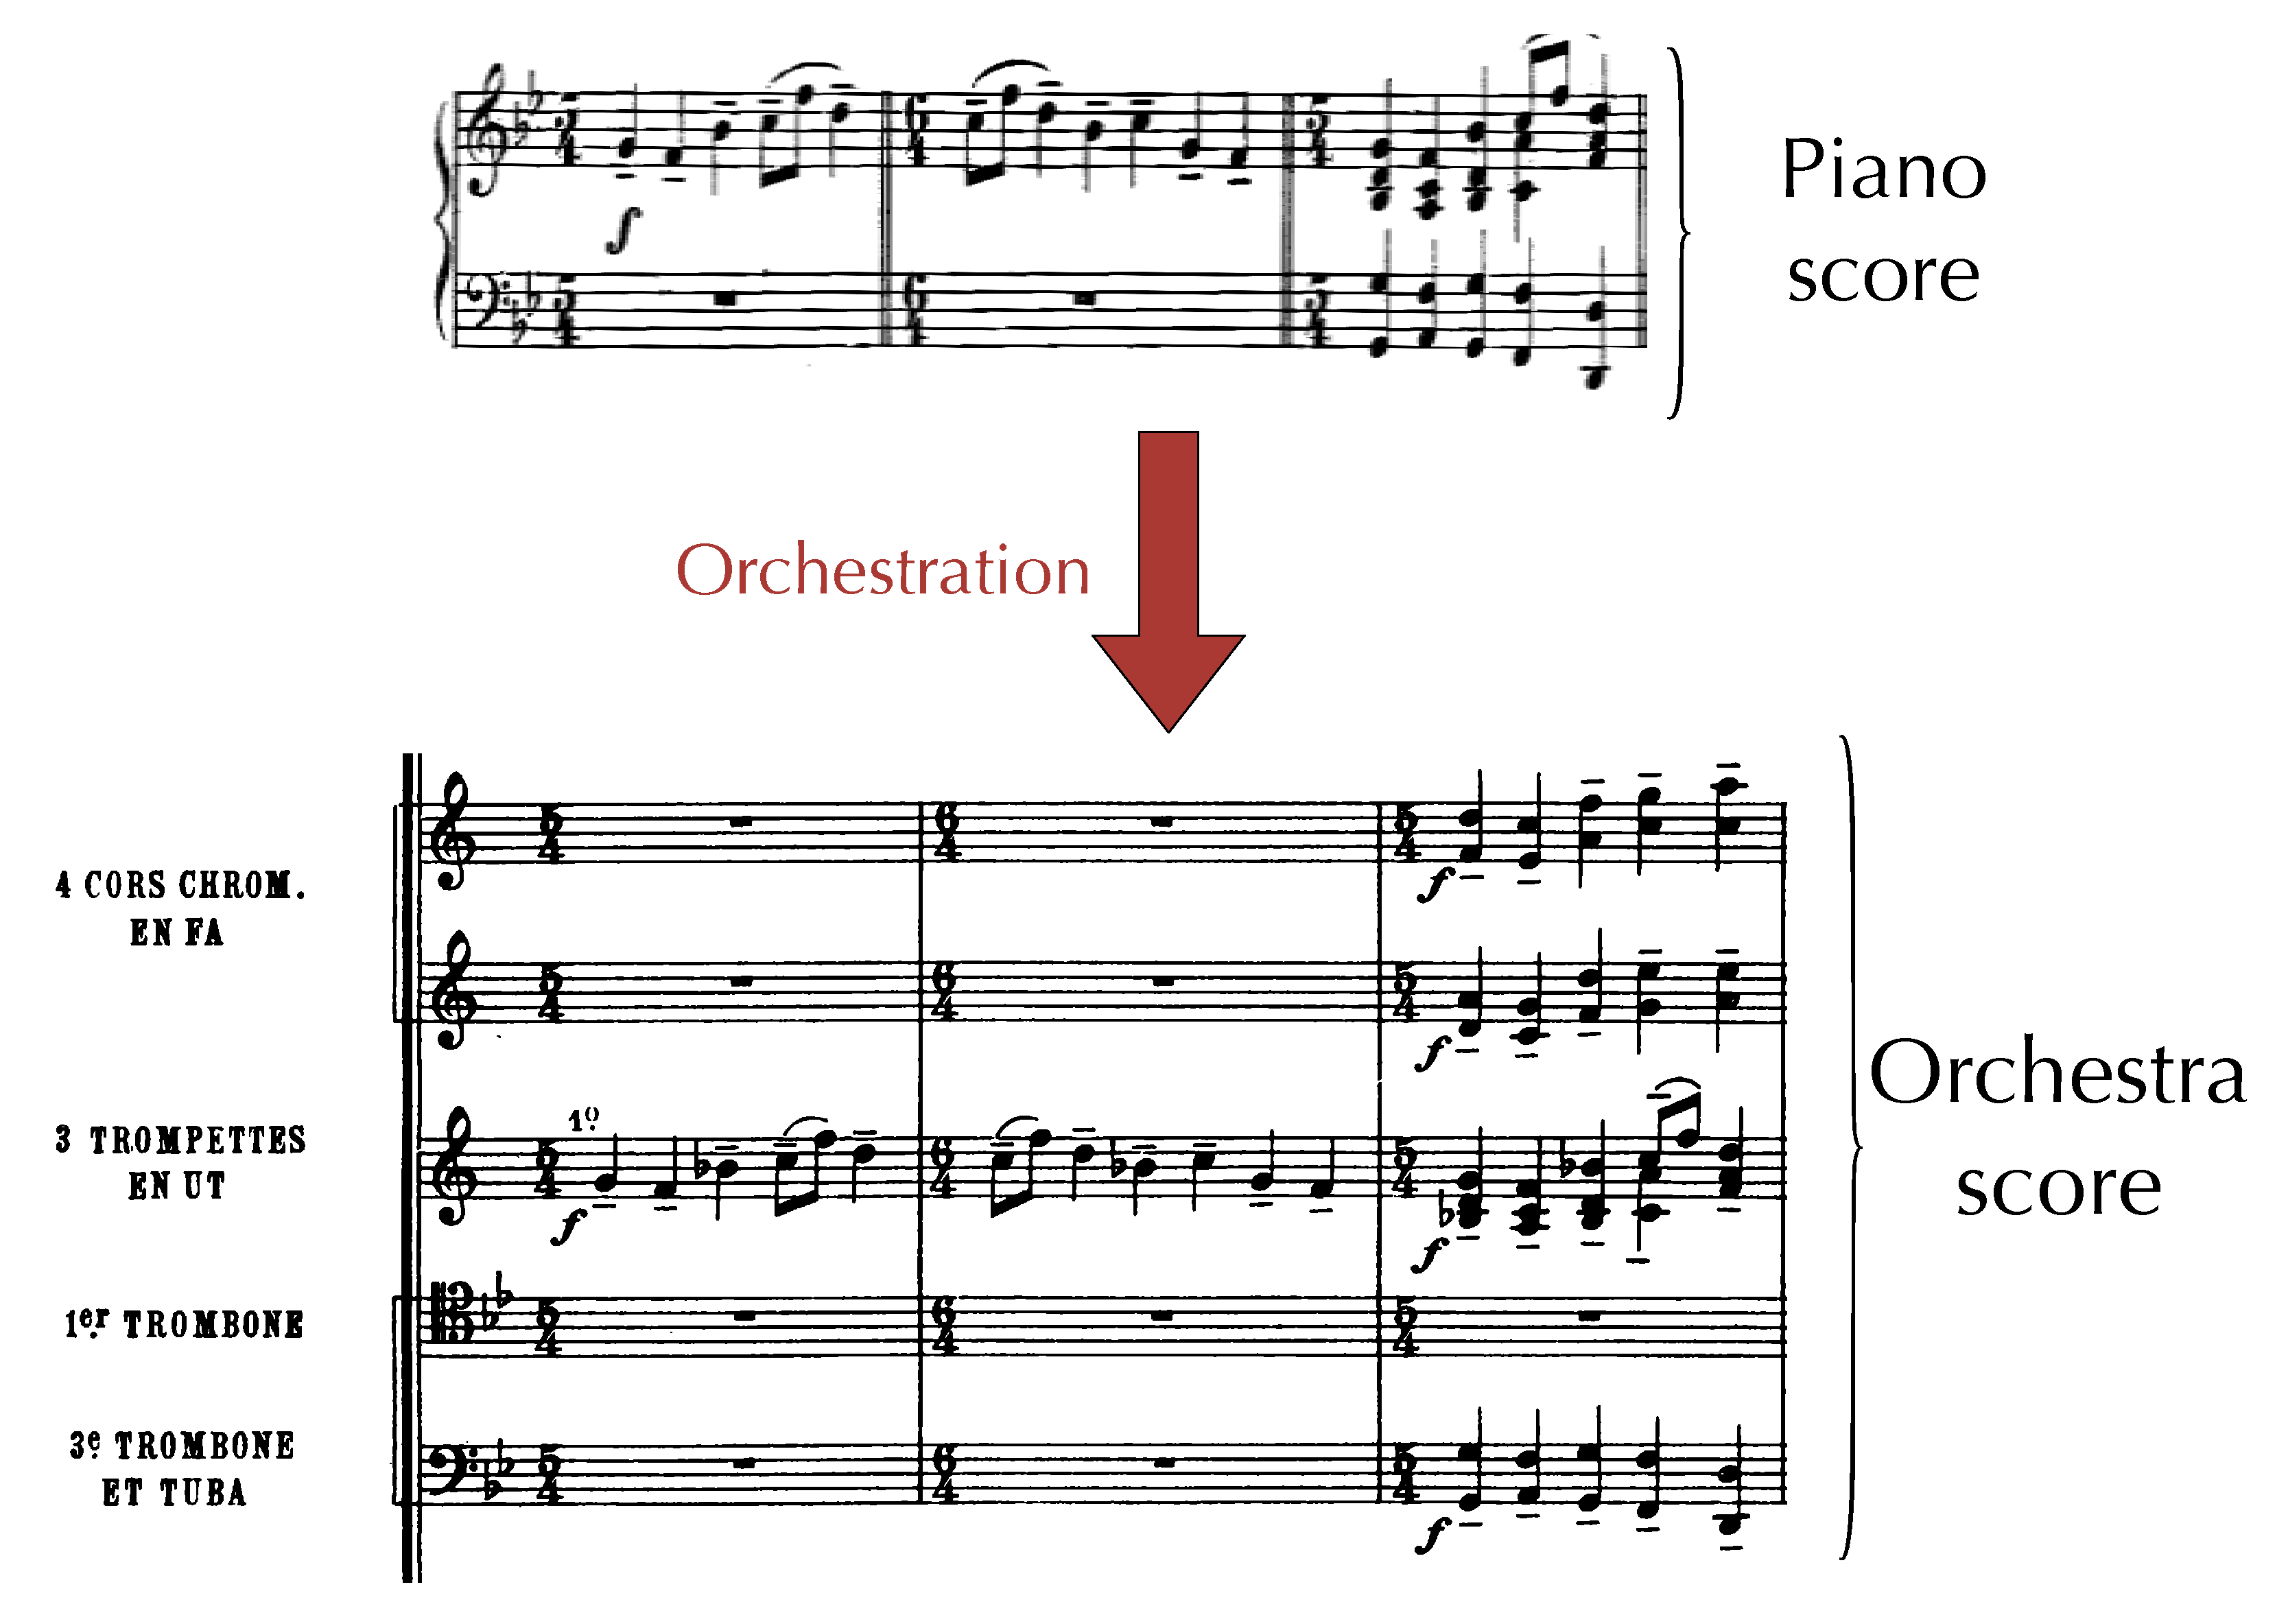
\includegraphics[scale=0.15]{Data_representation/orch}
\caption{\textit{Projective orchestration}. A piano score is projected on an orchestra. Even though a wide range of orchestrations exist for a given piano score, all of them will share strong relations with the original piano score. One given orchestration implicitly embeds the knowledge of the composer about timbre and orchestration.}
\label{fig:orch}
\end{figure}

Statistical inference covers a range of methods aimed at automatically extracting a structure from observations. These approaches hypothesize that a particular type of data might be structured by an underlying probability distribution. The objective is to deduce properties of this distribution, by observing a set of those data. 
If the structure of the data is efficiently extracted and organized, it should be possible in turn to generate novel examples.
%Thus, our objective is to build a system of automatic projective orchestration. 
We believe that learning the underlying distribution of a corpus of piano scores and their orchestrations by famous composers through statistical inference is a promising lead toward the automatic generation of orchestrations with a sensible timbre structure.
In the context of projective orchestration, the data are defined as the scores, formed by a series of pitches and intensities for each instrument. The set of observations is the set of projective orchestrations performed by famous composers, and the probability distribution would model the set of notes played by each instrument conditionally on the corresponding piano score.

It might be surprising at first to rely solely on symbolic information (scores) whereas we insisted on the fact that orchestration is the art of timbre, typically not represented in the musical notation but rather conveyed in the signal information (audio recording).
However, we make the assumption that spectrally consistent orchestrations could be generated from a purely symbolic learning by uncovering the composers' knowledge about timbre embedded in the score. As we rely on the works of composers that effectively took into account the subtleties of timbral effects, these symbolic relationships embed the spectral information.

A wide range of statistical inference models have been devised, among which deep learning recently appeared as a  promising field in artificial intelligence and representation learning \cite{bengio2013representation,LeCun:2015aa}.
Deep learning techniques have already been successfully applied to several musical applications and neural networks are now the state of the art in most music information retrieval tasks \cite{humphrey2012moving,lee2011unsupervised,boulanger2013audio} and for speech recognition and synthesis \cite{hinton2012deep,DBLP:journals/corr/OordDZSVGKSK16}. Generative systems working with symbolic information (musical scores) also appeared as a prosper flourishing framework for deep learning models. Successful applications have been made to automatic music composition \cite{eck2002finding,lavrenko2003polyphonic,bosley2010learning,boulanger2012modeling,Johnson2015}
automatic harmonization \cite{Sun} and style transfer \cite{pachet2016joyful}. However, the automatic projective orchestration task has never been investigated using deep learning methods and this paper is the first attempt to do so.

The final objective of the model we are trying to build is to generate orchestrations from unseen piano scores.
Hence, to model the influence of the piano score over the orchestral score, we focus on a class of models called \textit{Conditional RBM} \cite{taylor2006modeling}. To model the temporal structure of the orchestral scores, we exploit recurrent neural networks \cite{sutskever2013training}. We propose in this article to investigate several models belonging to those two classes and models combining elements from both types. \textbf{LIST ??}

In order to rank the different models, it is important to devise a quantitative evaluation framework. Designing a criterion assessing the performance of a generative model is a major difficulty for creative systems. In the polyphonic music generation field, a predictive task is commonly used \cite{boulanger2012modeling,lavrenko2003polyphonic,DBLP:journals/corr/YaoCVDD15}. Relying on these works, we introduce a specific framework for projective orchestration and made a benchmark of the introduced models in this framework. We then propose a qualitative analysis of both the models and the evaluation framework to explain the results obtained.

Finally, using the defined performance criterion we selected the most efficient model and implemented it in a system called \textit{Live Orchestral Piano} (LOP), an interface for real-time orchestration from a piano input.

The remainder of this paper is organized as follows. The section 2 is dedicated to the presentation of the different models investigated in this work. 
They all rely on the same training process that we describe at the beginning of the section. Then, the application of this training process to the different models is detailed, with an emphasis on the model we designed.
The projective orchestration task is presented in the section 3 along with an evaluation framework based on an event-level accuracy measure. The results of the introduced models along with their interpretation is proposed. Then (section 4), we introduce \textit{LOP}, the real-time projective orchestration system. Finally, we provide our conclusions and directions of future work.

\section{A training procedure for projective orchestration}
% Automatic orchestration ?
% On s'intéresse à des modèles par apprentissage.
% Quelle données ?
% Quelle fonction de coût ?
% Quelles architecture ?
The objective of this paper is to investigate the ability of a set of neural networks models to perform a projective orchestrations of a piano score. 
Neural networks are parametric models. These parameters need to be \textit{tuned} through a learning procedure.
A training procedure essentially consists in two things : data, which can be decomposed in a dataset and a data representation, and a error function. Then, tuning a neural networks means finding the set of parameters for which this error function is the lowest. Defining an error criterion in the context of projective orchestration is a sensitive question. We detail the predictive criterion we decided to use at the end of this section.

\subsection{Database}
We use a \textit{MIDI} database of piano scores and their orchestration by famous composers. A total of 223 pairs of piano score and corresponding orchestration have been collected and \textbf{??} different instruments are represented. 
Following the standard notations, all instruments of the same section are grouped under one unique part in the score. For instance, the \textit{violin} section, which might be composed by several instrumentalists, is written as a single part.
The database is available on this page \textbf{LINK}, along with a detailed description.

\subsection{Data representation}
\subsubsection{Orchestral Piano-roll}
In order to process the scores, we import them as matrices called \textit{piano-roll}, a data representation traditionally used to model polyphonic music of a single instrument (see \prettyref{fig:piano-roll}). 
Its extension to represent an orchestra is straightforwardly obtained by the concatenation of the \textit{piano-rolls} of each instrument along the pitch dimension.
In order to reduce the number of units, we systematically remove, for each instrument, any pitch which is never played in the training database. Hence, the dimension of the orchestral vector decreased from \textbf{2432} to \textbf{456}.

\begin{figure}[ht]
\centering
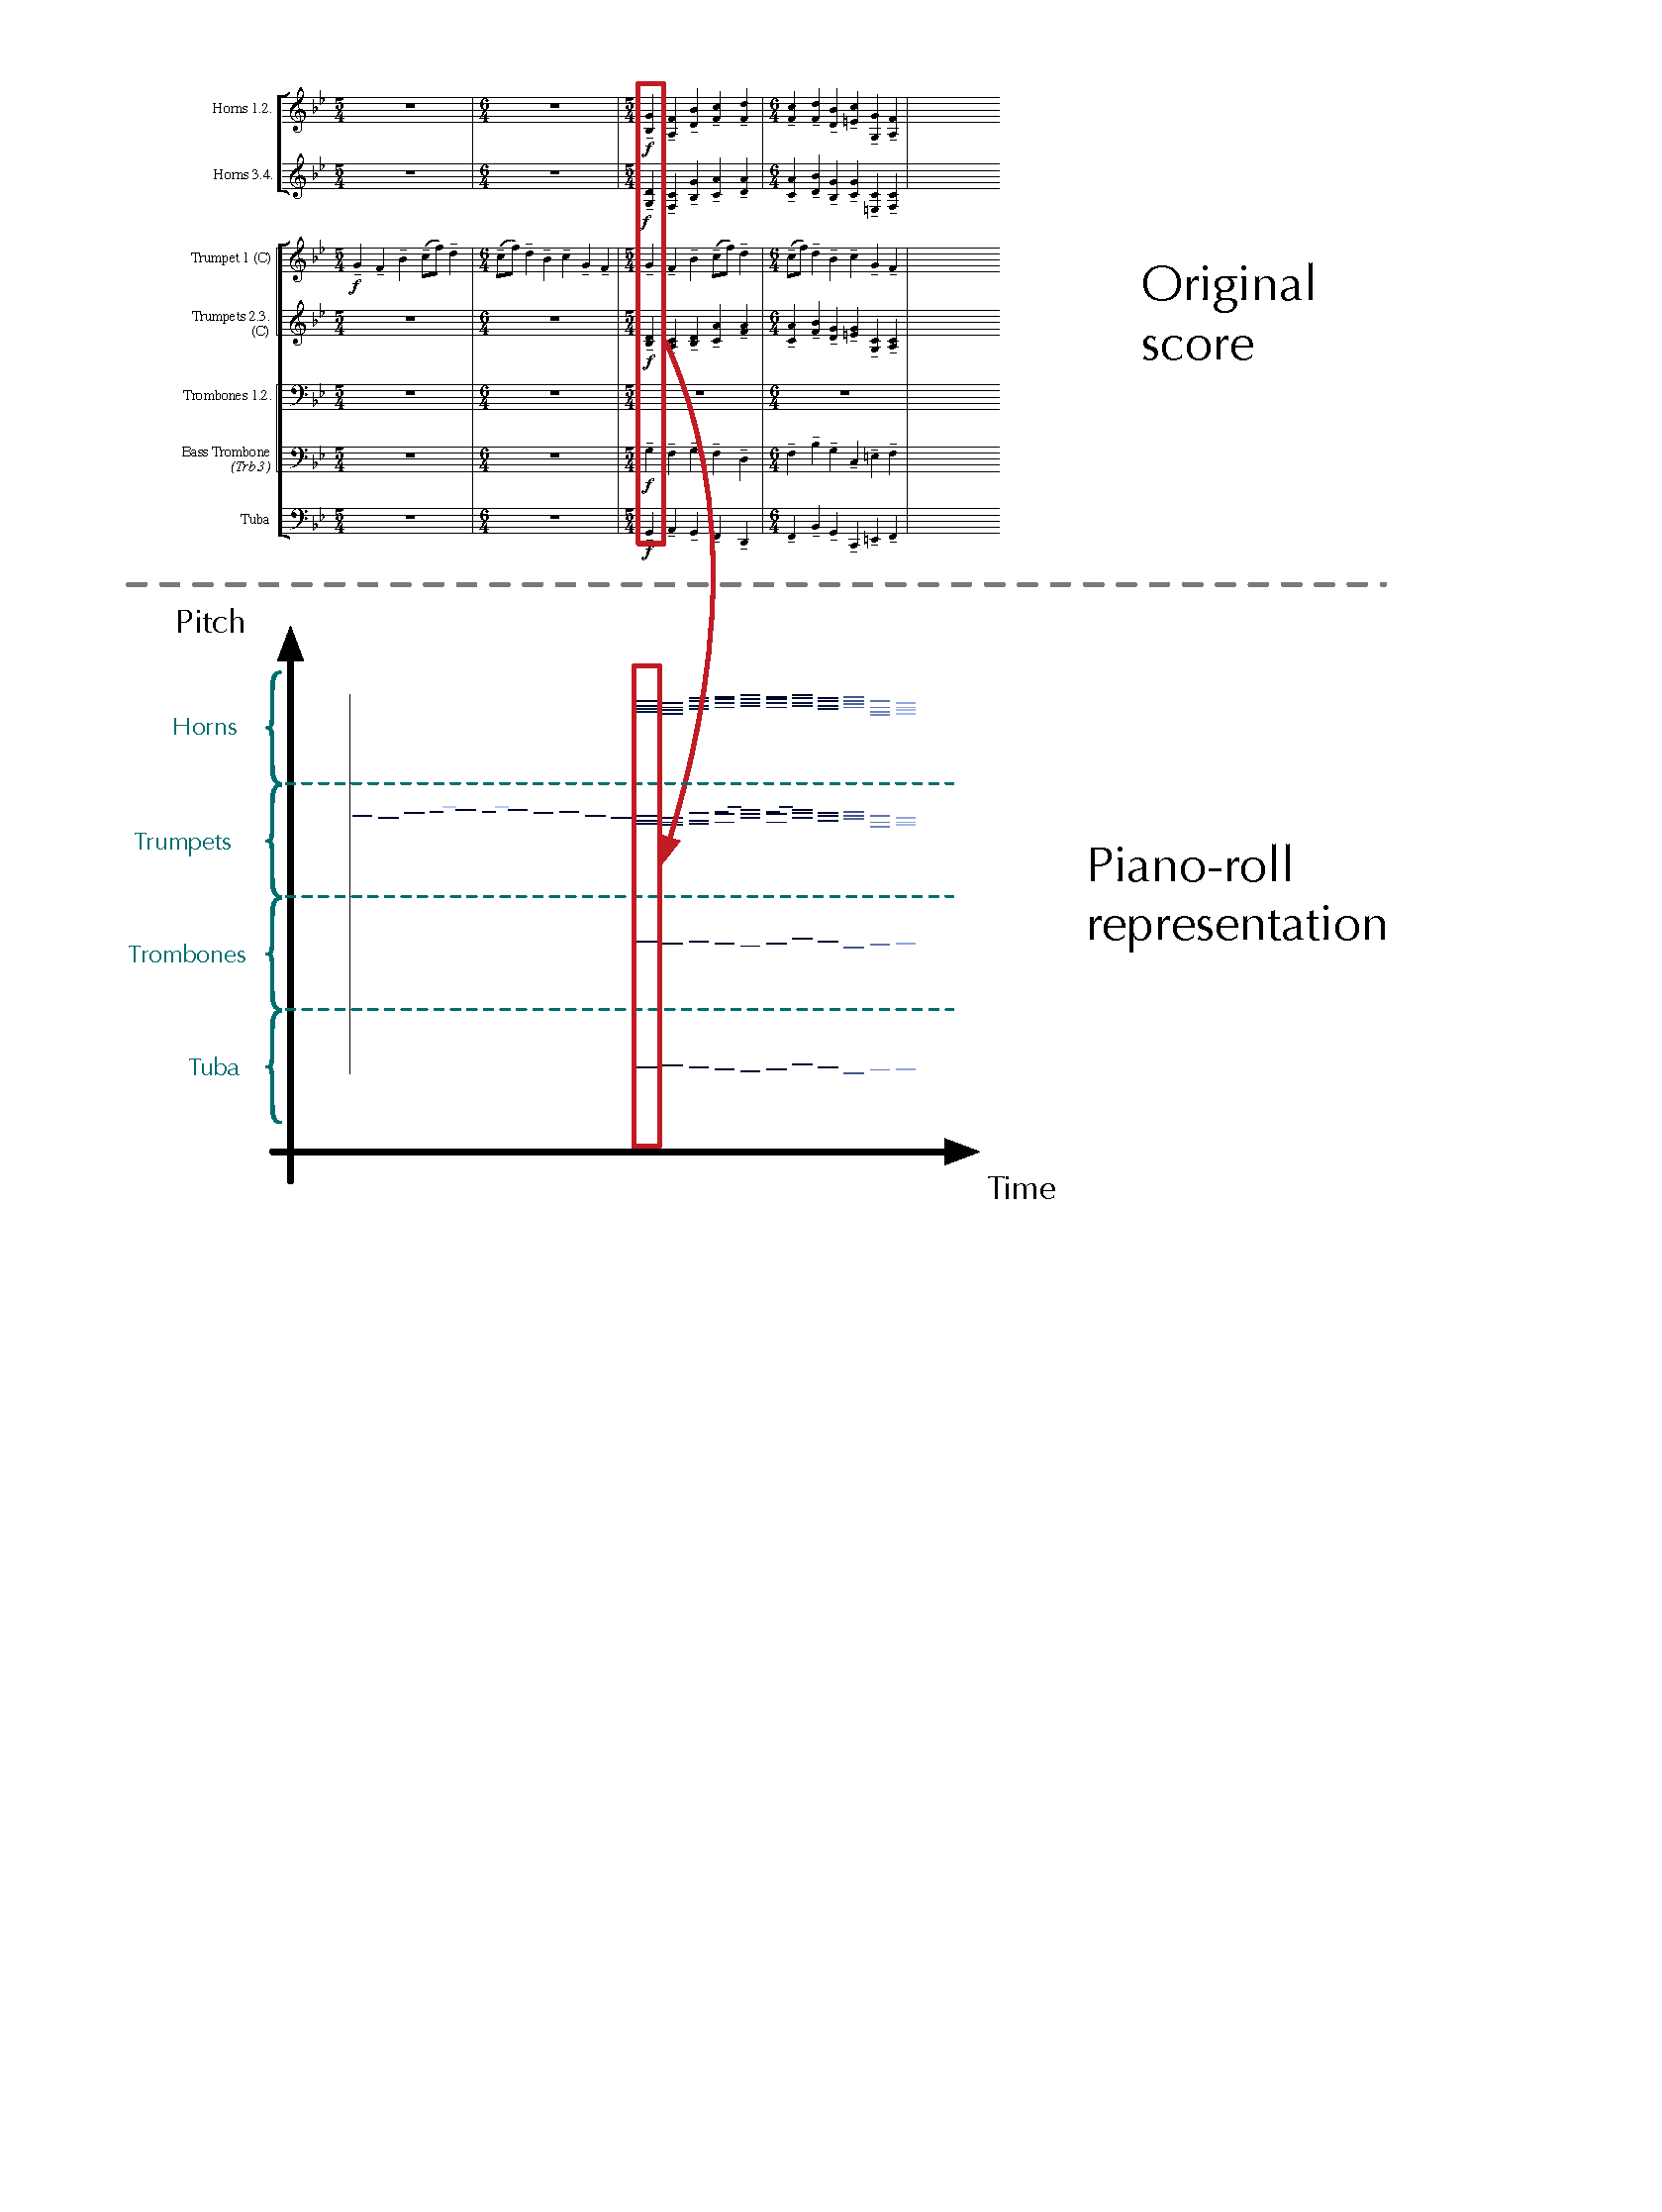
\includegraphics[scale=0.37]{Data_representation/from_score_to_pianoroll}
\caption{From the score of an orchestral piece, a convenient representation for computer processing named \textit{piano-roll} is extracted. A piano-roll $pr$ is a matrix whose rows represent pitches and columns represent a time frame depending on the time quantization. A pitch $p$ at time $t$ played with an intensity $i$ is represented by $pr(p,t) = i$, $0$ being a note off. This definition is extended to an orchestra by simply concatenating the \textit{piano-rolls} of every instruments along the pitch dimension.}
\label{fig:piano-roll}
\end{figure}

\subsubsection{Temporal granularities}
We defined two \textit{temporal granularities}.
\begin{itemize}
\item The \textit{frame-level granularity} consists in taking each successive frame into consideration in the piano-roll representation. The rhythmic quantization is defined as the number of time frame in the \textit{piano-roll} per quarter note and defines the precision of the frame-level representation.
\item The \textit{event level granularity} consists in conserving only the frames of the piano-roll representation where an event occurs. We define an event as a time $t_{e}$ where $\text{Orch}(t_{e}) \neq \text{Orch}(t_{e} - 1)$.  
% effet : plus de rhythme
Hence, the temporal precision of the event-level representation no longer depends on a quantization parameter and the scores are seen as a succession of events with no rhythmic structure.
% Justification
It can be justified by considering the simplified case where the rhythmic structure of the projected orchestral score is exactly the same as the one of the original piano score. 
This is false in the general case, since a composer can decide to add non-existent event in an orchestration, but it is a reasonable simplification.
\end{itemize}
In the result section, we discuss the impact of both representation over the performances of the different models \textbf{REF RESULTS SECTION}.
\textbf{SCHEMA}

\subsubsection{Dynamics}
Finally, the velocity information is discarded. Indeed, we use binary units which solely indicate if a note is on or off. We know that the velocity information is crucial in order to perform orchestration, since it can impact for instance the number of played instruments. However, we believe that the relative rank of the different architectures would not be deeply affected by considering intensities. Thus, the binary framework is a first step to discriminate relevant features amongst the different models.

\subsection{Training objective}
\subsubsection{Error function}
For each orchestral piece, we define $O$ and $P$ as the sequences of column vectors from the \textit{piano-roll} of the orchestra and piano parts, with $t \in \left[ 1,N_{T} \right]$ where $N_{T}$ is the length of the musical piece, given a particular quantization.

The objective is to design a function that is able to infer the present orchestral frame knowing the recent past of the orchestra sequence and both the past and present of the piano sequence. Mathematically, it consists in designing an \textit{inference function} $f$ where
\begin{equation}
\begin{aligned}
\hat{O}(t) = \bm{f}\lbrack & O(t-1), ..., O(t-N), & \\
	& P(t), ... ,P(t-N) \rbrack & \forall t \in \left\lbrack|1, ... N_{T}|\right\rbrack\\
\end{aligned}
\label{eq:inference_function}
\end{equation}
$N$ defines the order of the model. A model with a larger order is expected to perform better.

\subsubsection{Gradient descent}
\textbf{In the following section, we propose several implementations of the inference function $f$ as a neural network.
As neural networks are parametric models, the function $f$ also depends on a set of parameter $W$. For a given architecture, the best set of parameter has to be found through the iterative minimization of an error function $E$.
In the next section we describe the different error functions that are adapted for each model.
But in all cases, it depends on the distance between the predicted frame $\hat{O}$ and the original frame in the score $O$. Since $\hat{O}$ is inferred from the model, the error function depends on the parameter $W$.
Thus, a given parameter $w \in W$ is iteratively modified by a function of the partial derivative of $E$ with respect to $w$
\[
w_{new} = g(w_{old}, \frac{\partial E}{\partial w})
\]
} \textbf{A MON AVIS TOUT CA SERT A RIEN, ON DIT JUSTE : NEURAL NETS = MODEL PARAMETRIC -> GRADIENT DESCENT. ET SI LE LECTEUR NE SAIT PAS CE QUE C'EST, BAH IL LIT LA REF}
In this work, we used four different optimization methods for each model : gradient descent, RMS prop, Asam, Nesterov momentum.

\section{Neural networks}
Neural networks can be introduced in a probabilistic framework. The vectors $O(t)$ and $P(t)$ extracted from the piano-roll representation are modelled by sequences of random variables.
The models we explore express the conditional dependencies between the present orchestral vector $O(t)$, the present piano vector $P(t)$ and the past orchestral vectors $O(t-N),...,O(t-1)$. \textit{Hidden units} are introduced to model the co-activation of these variables and are often considered as an higher-level representation encoding the regularities of the raw data.

% Description générale : RBM, conditional, recurrent
Given the large number of models that recently flourished in the machine learning field, we decided to restrict the benchmark to models based on the Restricted Boltzmann Machine (\textit{RBM}).
The \textit{RBM} is the building block of many complex architectures. It is a generative models, which means that the model tries to reconstruct the hypothetical probability distribution of the data observed in the training database.

We further reduce the number of model by considering only those which implement a notion of conditional dependence or temporal recurrence. The recurrences model the temporal structure of the orchestral score (influence of $O(t-N),...,O(t-1)$ on $O(t)$. Ideally, the conditional dependences represent the influence of the piano score over the orchestral score ($P(t)$ over $O(t)$), but also the temporal dependencies in some models.

Those architectures are quickly introduced in the following section and we insist on the application of those models to the case of projective orchestration. For detailed descriptions, references to the original papers are provided. The names of the models are : Restricted Boltzmann Machine (\textit{RBM}), conditional RBM (\textit{cRBM}), Factor Gated cRBM (\textit{FGcRBM}), recurrent network with Long short-term memory units (\textit{LSTM}) and Recurrent neural network RBM (\textit{RnnRBM}).
We also propose and detail two hybrid architectures called conditional RnnRBM (\textit{cRnnRbm}) and Factored Gated cRnnRBM (\textit{FGcRnnRbm}).

\subsection{Restricted Boltzmann Machine}
\subsubsection{An energy based model}
% Energy -> probability
A RBM models the joint probability of visible and hidden random variables by $p_{model}(\bm{v},\bm{h}) = \frac{\exp^{-E(\bm{v},\bm{h})}}{Z}$ where
\begin{equation}
\label{eq:energy}
E(\bm{v},\bm{h}) = - \sum_{i=1}^{m} a_{i} v_{i}  - \sum_{i=1}^{m} \sum_{j=1}^{n} v_{i} W_{ij} h_{j} - \sum_{j = 1}^{n} b_{j} h_{j}
\end{equation}
with $\Theta = \left\{W,b,a\right\}$ the parameters of the network.
In the case of projective orchestration, the visible units are defined as the concatenation of the past and present orchestra and the present piano 
\begin{equation}
\label{eq:visible_rbm}
\bm{v} = \left[P(t),O(t-N),...,O(t)\right]
\end{equation}

\begin{figure}[h]
\centering
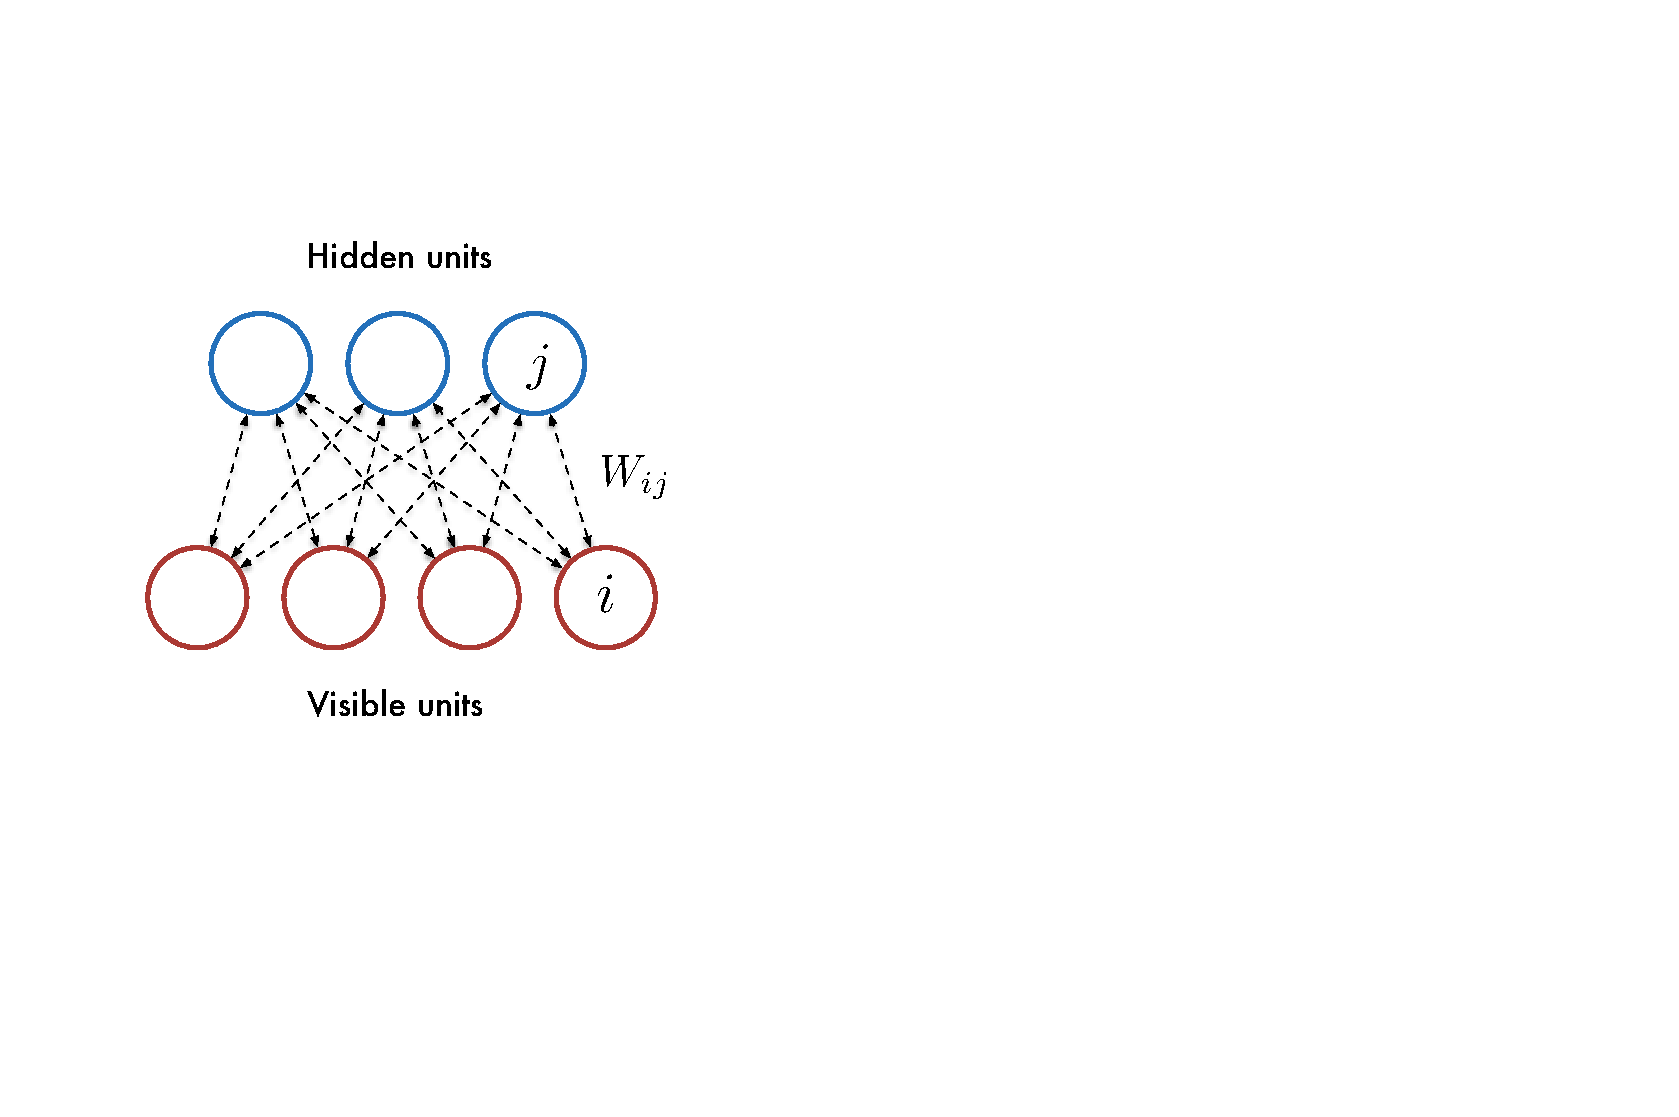
\includegraphics[scale=0.6]{RBM}
\caption{\textbf{Modifier la figure pour qu'apparaissent past orch, present piano, present orch}
The \textit{Restricted Boltzmann Machine} (RBM) is defined by a set of visible ($v_{i}$) and hidden ($h_{j}$) units. Symmetric weights ($W_{ij}$) connect a hidden unit to a visible unit which altogether define an energy function $E_{W}(v,h)$. Training an \textit{RBM} consists in modifying the weights $W$ to lower the energy function around the points observed in the training set.}
\label{fig:RBM}
\end{figure}
\subsubsection{Training in a RBM}
% A typical cost function = likelihood
A popular and well suited error function to train probabilistic models is the negative log-likelihood 
\begin{equation}
\label{eq:likelihood}
\mathcal{L(\bm{\theta}|\mathcal{D})}  = \frac{1}{N_{\mathcal{D}}} \sum_{\bm{v^{(l)}} \in \mathcal{D}} - \ln \left( p(\bm{v^{(l)}}|\bm{\theta})\right)
\end{equation}
where $\mathcal{D}$ is the training dataset, $N_{\mathcal{D}}$ its size. The size is the number of visible vectors that can be constructed as in \prettyref{eq:visible_rbm}. This number depends on the number of files and the order $N$ of the model.

% Likelihood ? Intractable
Ideally, the training procedure consists in modifying the parameters $\Theta$ of the model along the gradient of the error function.
However, the gradient of negative log-likelihood is intractable,
% Contrastive divergence
and an approximation of this quantity is used instead. This technique is called contrastive divergence (\textit{CD}) \cite{fischer2012introduction,hinton2010practical}.
\subsubsection{Generating}
% Computing p(x) ?
% = negative particule of the CD !!
% Pbm, in the case of RBM simple generate piano + orchestra -> generation through inpainting
% Mais du coup, c'est un peu con de modéliser le piano pour pas l'utiliser non ?

\subsection{Conditional models}
% Un moyen de tej le piano de la function d'energie = conditional models. En fait, c'est un peu comme clamper en permanence, même durant la training step, le piano.
\subsubsection{Conditional RBM}
\subsubsection{Factored Gated cRBM}
% Gated = dissocier la contribution du passé et l'influence du piano
% Factor = Solve computations problèmes (tensor mega huge)
% Mais est-ce qu'on a pas des modèles temporels plus adaptés ?

\subsection{Recurrent networks}
% Et que si
\subsubsection{LSTM}
\subsubsection{RnnRbm}
% Même des modèles génératifs

\subsection{Conditional recurrent architectures}
\subsubsection{cRnnRbm}
\subsubsection{FGcRnnRbm}

\section{Evaluation framework}
In this section, we introduce and formalize the automatic projective orchestration task presented in \prettyref{fig:orch}. In particular, we detail the database and data representation used, evaluation framework, and discuss the results obtained by different models.

\subsection{Evaluation framework}
We introduce an \textit{event-level orchestral inference} task to evaluate our models. To our best knowledge, this is the first attempt to define a quantitative evaluation framework for automatic projective orchestration.

In order to evaluate the models, the data used to train and those used to assess the performances must be different \cite{bishop2006pattern}. Hence, the dataset is usually split between a train and test set.
Given the complexity of the distribution we want to model and the extremely narrow size of the database, we rely on a Leave-One-Out (\textit{LOO}) evaluation where 75 scores are used to train the model and one is kept for testing. This choice is motivated by the will to obtain the best generative model possible.

Predictive symbolic music tasks are usually evaluated through a \textit{frame-level} accuracy measure where each time frame of the piano-roll is considered as a separate data example \cite{DBLP:journals/corr/YaoCVDD15,boulanger2012modeling,lavrenko2003polyphonic}.
We propose to work in an \textit{event-level} framework, where data examples are only those for which an event occurs. An event is defined as a time $t_{e}$ where $\text{Orch}(t_{e}) \neq \text{Orch}(t_{e} - 1)$. The reason why we do not rely on a \textit{frame-level} evaluation is that a model which simply repeats the previous frame gradually becomes the best model as the quantization gets finer. Moreover, in the projective orchestration framework, rhythmic patterns are already established by the known piano score and, thus, does not have to be learned by the model.

% Nombre de batch
Finally, to speed-up the convergence of the gradient descent, mini-batches are used to train the model \cite{bishop2006pattern}. Following these procedures, 89 mini-batches of 100 event-level points were obtained for training.

\subsection{Measure}
An objective criterion of the performances of the models is necessary to provide an evaluation. 
The best way for evaluating generative models is to compute the likelihood of the test set (see equation \prettyref{eq:likelihood}). However, we have seen that this quantity is intractable in all \textit{RBM}, \textit{cRBM} and \textit{FGcRBM} models. 
An alternative criterion commonly used in the music generation field is the accuracy measure \cite{DBLP:journals/corr/YaoCVDD15,boulanger2012modeling,lavrenko2003polyphonic}. For each \textit{event} $t_{e}$ (see previous section), the visible units of the model are sampled with its context (and features for the FGcRBM) units set to $Orch(t_{e}-1),... Orch(t_{e}-N)$ and $Piano(t_{e})$ from the test dataset. This sampled prediction $\text{Pred}(t_{e})$ is then compared to the ground-truth vector $\text{Orch}(t_{e})$ from the test dataset via the accuracy measure
\begin{equation}
\text{Accuracy}  = \frac{TP(t)}{TP(t) + FP(t) + FN(t)}
\label{eq:accuracy}
\end{equation}
where $TP(t)$ (true positives) is the number of notes correctly predicted (note played in the prediction and ground-truth). $FP(t)$ (false positive) is the number of notes predicted which are not in the original sequence (note played in the prediction, but not in ground-truth). $FN(t)$ (false negative) is the number on unreported notes (note absent in prediction, but played in ground-truth). 
Instead of binary values, activation probabilities are used for the predicted samples in order to avoid sampling noise.

\subsection{Results}
Four models are evaluated on the orchestral inference task. The first model is a random generation of the orchestral frames from a Bernoulli distribution of parameter $0.5$. The second model predicts an orchestral frame at time $t$ by repeating the frame at time $t-1$. Those two naive models constitute a first baseline against which we compare the cRBM and FGcRBM models.

The results are summed up in \prettyref{tab:result_event_level}. As expected, the random model has poor results. The repeat model performs significantly better. Indeed, it is relatively common that a note is sustained between two successive events. The cRBM largely outperforms those two models. However, the FGcRBM model has a lower score than the repeat model. We observed that the activation function of the visible units during the generative step was extremely noisy, which suggests that the training procedure mostly failed. We believe that this is due to the number of parameter,  and especially the dimension of the feature units. Indeed, in \cite{taylor2009factored}, only ten different configuration of the feature units were possible. When training on an orchestral database,  each different piano frame define a different configuration.

\begin{table}[h]
\centering
\begin{tabular}{c c c}
\hline
\thead{Model} & \thead{Frame-level\\ accuracy} & \thead{Event-level\\ accuracy} \\
\hline
Random & ? & ?\\ 
Repeat & ? & ?\\
\hline \hline
RBM & ? & ?\\ 
cRBM & ? & ?\\ 
FGcRBM & ? & ?\\ 
LSTM & ? & ?\\
RnnRbm & ? & ?\\ 
cRnnRbm & ? & ?\\ 
FGcRnnRbm & ? & ?\\ 
\end{tabular}
\caption{Event-level and frame-level (with quantization 4) accuracy for the orchestral inference task.}
\label{tab:result_event_level}
\end{table}

\subsection{Discussion : evaluating a generative model ?}
It is important to state that we do not consider this predictive measure as as reliable measure of the creative performance of a model. Indeed, predicting and creating are two fairly different things. 
Hence, the predictive evaluation framework we have built does not assess the generative ability of a model, but is rather used as a selection criterion among different models.

%As pointed out in \cite{boulanger2012modeling}, a better evaluation measure would be the likelihood of a sequences from a test dataset. Unfortunately, these quantities are computationally intractable in the introduced models. However, recent works estimator of the partition function 
%
%\section{Live Orchestral Piano (LOP)}
%We introduce in this section the \emph{Live Orchestral Piano} (LOP)
%application, which is the first software able to provide a way to
%compose music with a full classical orchestra in real-time by simply
%playing on a MIDI piano. The goal of this framework is to rely on
%the knowledge learned by the model introduced in the previous sections
%in order to perform the projection from a piano melody to the orchestra.
%
%\subsection{Workflow}
%The software is implemented on a client/server paradigm. This choice
%allows to separate the orchestral computation part from the interface
%and sound rendering engine. That way, multiple interfaces can easily
%be implemented. It should also be noted that separating the computing
%and rendering on different computers, can allow to use high-quality
%and CPU-intensive orchestral rendering plugins. This can allow a more
%realistic orchestral rendering with heavy amounts of computation performed
%while ensuring the real-time constraint on the overall system (preventing
%degradation of the computing part). The complete implementation workflow
%is presented in Figure~\ref{fig:Live-orchestral-piano}.
%
%\begin{figure*}
%\begin{centering}
%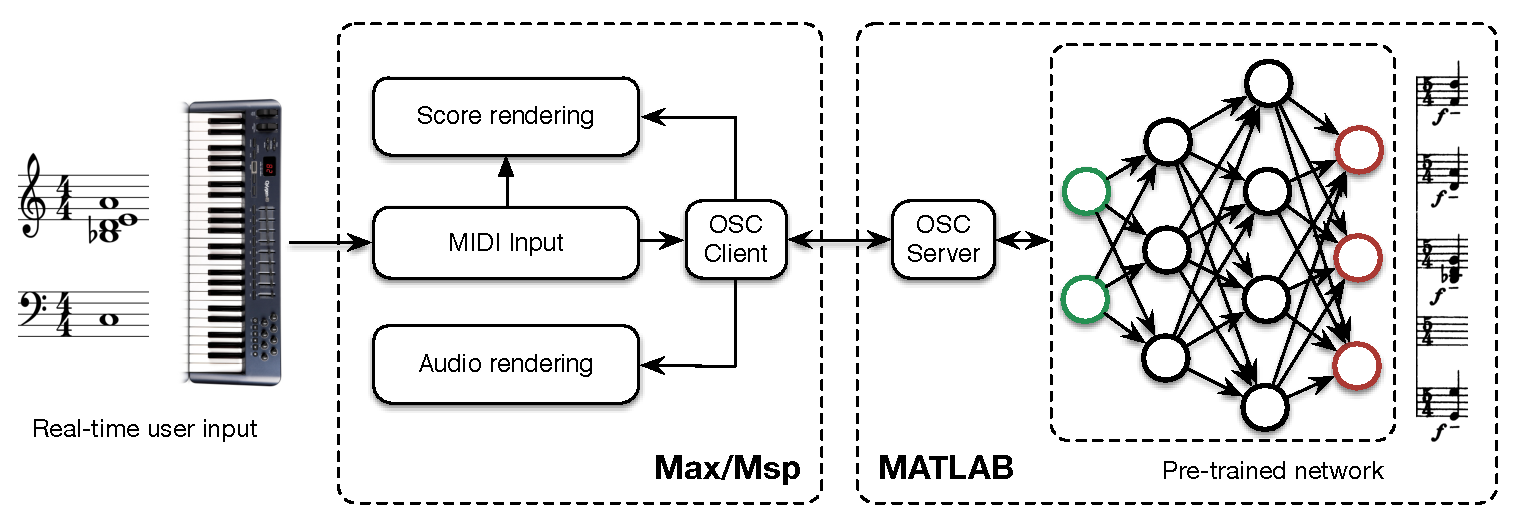
\includegraphics[scale=0.55]{workflow}
%\par\end{centering}
%
%\caption{\label{fig:Live-orchestral-piano}Live orchestral piano (L.O.P) implementation
%workflow. The user inputs a melody which is transcribed into a score
%and send via OSC from the Max/Msp client. Then, the MATLAB server
%uses this vector of notes and process it following the aforementioned
%techniques in order to obtain the orchestration. This information
%is then sent back to Max/Msp which performs the real-time audio rendering }
%\end{figure*}
%
%As we can see, the user can input a melody (single notes or chords)
%through a MIDI keyboard, which is retrieved inside the Max/Msp interface.
%The interface transmits this symbolic information (as a variable-length
%vector of active notes) via OSC to the MATLAB server. The interface
%performs a real-time transcription of the piano score to the screen
%in parallel. The server uses this vector of events to produce an 88
%vector of binary input note activations (as defined in the sub-section \textit{Data representation}).
%This vector is then processed by using the orchestration algorithms
%presented in sub-section \textit{Model definition} in order to obtain a projection
%of a specific symbolic piano melody to the full orchestra (an operation
%defined as \emph{projective orchestration}). The resulting orchestration
%is then sent back to the client interface which performs both the
%real-time audio rendering and score transcription. 
%
%\subsection{Interface}
%The interface has been developed in Max/Msp, to facilitate both the
%score and audio rendering aspects in a real-time environment. The
%score rendering is handled by the \emph{Bach} library environment. 
%This interface provides a way to easily switch between different orchestration models, while controling other
%meta-parameters of the sampling. For instance the \emph{cutoff probability
%}gives a direct access to the density of the generated orchestration
%(in terms of number of played instruments). Indeed, a low cutoff probability
%implies that most activation of notes will be taken into account in
%the playback, while a high cutoff will produce more sparse orchestration.
%
%\section{Conclusion and future works}
%% Orchestral inf problem
%We have introduced a system for real-time projective orchestration of a midi piano input. In order to select the most adapted model, we have proposed an evaluation framework called orchestral inference which rely on an orchestral inference task. We have assessed the performance of the cRBM and FGcRBM, and observed the better performances of the cRBM model.
%
%% Interesting and highly benefit problem
%The general objective of building a generative model for time series is one of the most prominent topic for the machine learning field. Orchestral inference sets a slightly more specific framework where the generated time series is conditioned by an other observed time series (the piano score). Besides, being able to grasp the long range dependencies structuring music appears as a challenging and worthwhile task.
%
%% Increase DB
%The high dimensionality of the data and their sparsity are a major obstacle for learning algorithms.
%A first remark is that a larger database would be required to train any model sufficiently complex to properly represent the underlying distribution of a projective orchestration.
%It is important to build a reference database of piano scores and their orchestration by acknowledge composers, with all instrument name indicated and velocity for the notes. 
%% Velocities
%Indeed, we believe that taking the notes' velocity into consideration is crucial, since many orchestral effects are justified by intensity variations in the original piano scores. 
%% Find distrib representations
%Besides, the sparse representation of the data suggests that a more compact distributed representation might be found. Lowering the dimensionality of the data would greatly improve the efficiency of the learning procedure. For instance, methods close to the word-embedding techniques used in natural language processing might be useful \cite{kiros2015skip}.
%
%Finally, a better performance measure should be developed for the orchestral inference task. A solution could be to derive estimators for the likelihood of sequences under the proposed models. Recent work on methods such as Annealed Importance Sampling are promising.

\section{Acknowledgements}
This work has been supported by the \textit{NVIDIA GPU Grant} program.
The authors would like to thank Denys Bouliane for kindly providing the orchestral database.

%%%%%%%%%%%%%%%%%%%%%%%%%%%%%%%%%%%%%%%%%%%%%%%%%%%%%%%%%%%%%%%%%%%%%%%%%%%%%
%bibliography here
\bibliography{../Biblio/biblio}

\end{document}
